\chapter{Kajian Pustaka}

Bab Kajian Pustaka digunakan untuk mendeskripsikan kajian literatur yang terkait dengan persoalan tugas akhir. Tujuan kajian pustaka adalah:
\begin{enumerate}
\item memberikan pemahaman yang cukup kepada pembaca tentang teori atau pekerjaan yang terkait langsung dengan penyelesaian persoalan

\item menyampaikan informasi apa saja yang sudah ditulis/dilaporkan oleh pihak lain (peneliti/Tugas Akhir/Tesis) tentang hasil penelitian/pekerjaan mereka yang sama/mirip/erat kaitannya dengan persoalan tugas akhir

\item menunjukkan kepada pembaca adanya gap seperti pada rumusan masalah yang memang belum terselesaikan
\end{enumerate}

\section{Contoh Subbab}
Contoh subbab

\subsection{Contoh Subbab}
Contoh subbab.

\subsubsection{Contoh Gambar dan Tabel}
Contoh gambar adalah sebagaimana terlihat pada Gambar \ref{fig:eg}.
\begin{figure}
    \centering
    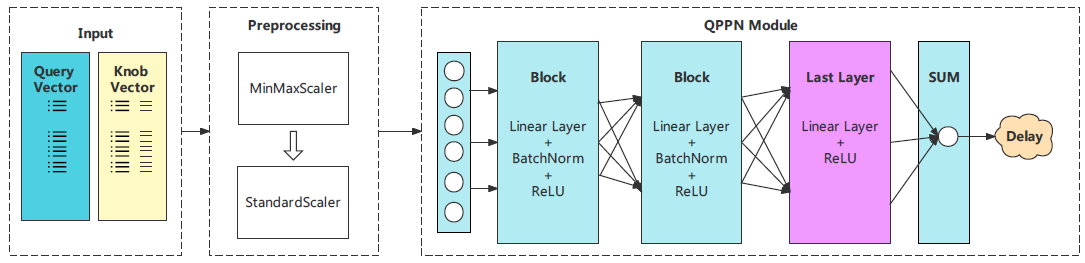
\includegraphics[width=0.8\linewidth]{images/QPPN.png}
    \caption{Tahapan konstruksi koleksi retorik kalimat}
    \label{fig:eg}
\end{figure}

Contoh tabel adalah sesuai yang terlihat pada Tabel \ref{tab:my_label}.
\begin{table}[]
    \centering
    \begin{tabular}{|l|l|}
    \hline
    Nomor \textit{Tag}  & Keterangan \\
    \hline
        0xx  & Kendali informasi, nomor dan kode\\
        \hline
        1xx & Main entry\\
    \hline
    \end{tabular}
    \caption{Pengelompokan \textit{Tag} MARC-21}
    \label{tab:my_label}
\end{table}